 \documentclass[10pt, table, dvipsnames,xcdraw, handout]{beamer}
\usetheme[progressbar=frametitle]{metropolis}
\usepackage{appendixnumberbeamer}
\usetikzlibrary{arrows.meta, positioning, quotes}
\usepackage[shortlabels]{enumitem}
\usepackage{xcolor}
\usepackage{mathtools}


\usepackage{cancel}

\newcommand\hcancel[2][black]{\setbox0=\hbox{$#2$}%
\rlap{\raisebox{.45\ht0}{\textcolor{#1}{\rule{\wd0}{1pt}}}}#2} 


\usepackage{booktabs}
\usepackage[scale=2]{ccicons}

\usepackage{pgfplots}
\usepgfplotslibrary{dateplot}

\usepackage{xspace}
\newcommand{\themename}{\textbf{\textsc{metropolis}}\xspace}
\newcommand{\cb}{\cellcolor{blue!25}}


% Notation:
\newcommand{\cT}{\ensuremath{\mathcal{T}}}
\newcommand{\cD}{\ensuremath{\mathcal{D}}}
\newcommand{\cX}{\ensuremath{\mathcal{X}}}
\newcommand{\cY}{\ensuremath{\mathcal{Y}}}
\newcommand{\cZ}{\ensuremath{\mathcal{Z}}}
\newcommand{\cH}{\ensuremath{\mathcal{H}}}
\newcommand{\cG}{\ensuremath{\mathcal{G}}}

\newcommand{\bR}{\ensuremath{\mathbb{R}}}
\newcommand{\bN}{\ensuremath{\mathbb{N}}}
\newcommand{\bP}{\ensuremath{\mathbb{P}}}
\newcommand{\bT}{\ensuremath{\mathbb{T}}}
\newcommand{\bL}{\ensuremath{\mathbb{L}}}

\newcommand{\bfX}{\ensuremath{\mathbf{X}}}
\newcommand{\bfY}{\ensuremath{\mathbf{Y}}}
\newcommand{\bfy}{\ensuremath{\mathbf{y}}}

\def\layersep{2.5cm}

% Tikz seys
\tikzset{cross/.style={cross out, draw, 
         minimum size=2*(#1-\pgflinewidth), 
         inner sep=0pt, outer sep=0pt}}

\title{Machine Learning I}
\subtitle{Lecture 10: Recurrent Neural Networks}
% \date{\today}
\date{}
\author{Nathaniel Bade}
\institute{Northeastern University Department of Mathematics}
% \titlegraphic{\hfill\includegraphics[height=1.5cm]{logo.pdf}}

\begin{document}

\maketitle

\begin{frame}{Table of contents}
  \setbeamertemplate{section in toc}[sections numbered]
  \tableofcontents[hideallsubsections]
\end{frame}


%%%%%%%%%%%%%% Slidshow Start %%%%%%%%%%%%%% 



\section{Types of Artificial Neural Networks}
\begin{frame}[fragile]{Genre of Artificial Neural Networks}
Modern artificial neural networks can be sorted into three broad categories based on their structure:

\begin{itemize}
\item[] Feed forward networks: A trained feed forward network acts like a function, taking in a set of data at one end and returning a new set of data at the other.\pause

\item[] Recurrent networks: Trained recurrent networks are stateful. That is, RNN's take data and return an output but the remember the last $M$ pieces of data sent through in an internal \textbf{state}. \pause

\item[] Symmetrically Connected Networks: A trained SCN is a densely connected network with an update rule. For any initial value of the nodes, the function ``updates," moving at each step towards a ``lower energy state". The result is achieved when updating no longer changes the sate. 
\end{itemize}
\end{frame}





\begin{frame}[fragile]{Feed Forward Networks}
  \begin{minipage}[t][0.5\textheight][t]{\textwidth}
	\centering \includegraphics[height=0.5\textheight]{L12FFNetwork.png} 
  \end{minipage}
  \vfill
\begin{minipage}[t][0.5\textheight][t]{\textwidth}
Feed forward networks are the most common type, they take an input, process it through a series of operation, and return some output. \newline\pause 

Mathematically they are just functions $f_\beta (X)$ depending on some trainable parameters $\beta$. They could result in a classifier $\hat{y} = f_\beta (X)$, or a loss function $\ell(X,z) = f_\beta (X)$. 
\end{minipage}
\end{frame}





\begin{frame}[fragile]{Feed Forward Networks}
  \begin{minipage}[t][0.5\textheight][t]{\textwidth}
	\centering \includegraphics[height=0.5\textheight]{L12Deconv.png} 
  \end{minipage}
  \vfill
\begin{minipage}[t][0.5\textheight][t]{\textwidth}
For example feed forward networks can be labeling or regression, but they can also be generative networks (returning more data) or unsupervised, returning a dimensional reduction, clustering or other description of the data. \newline \pause

However, once trained the weights $\beta$ are \textbf{fixed} for all prediction.
\end{minipage}
\end{frame}



\begin{frame}[fragile]{Recurrent Networks}
  \begin{minipage}[t][0.5\textheight][t]{\textwidth}
	\centering \includegraphics[height=0.5\textheight]{L12RNN.png} 
  \end{minipage}
  \vfill
\begin{minipage}[t][0.5\textheight][t]{\textwidth}
A recurrent neural network has state variables that can be changed at runtime and that persist between prediction runs.\pause\newline

For example, in text prediction an RNN may predict one word at a time while "remembering" its previous predictions. 
\end{minipage}
\end{frame}



\begin{frame}[fragile]{Recurrent Networks}
  \begin{minipage}[t][0.5\textheight][t]{\textwidth}
	\centering \includegraphics[height=0.5\textheight]{L12RNN2.png} 
  \end{minipage}
  \vfill
\begin{minipage}[t][0.5\textheight][t]{\textwidth}
A recurrent neural network on the other hand has state variables that can be changed at runtime and that persist between prediction runs.\newline

For example, in text prediction an RNN may predict one word at a time while "remembering" its previous predictions. 
\end{minipage}
\end{frame}




\begin{frame}[fragile]{Recurrent Networks}
  \begin{minipage}[t][0.5\textheight][t]{\textwidth}
	\centering \includegraphics[height=0.5\textheight]{L12RNN3.png} 
  \end{minipage}
  \vfill
\begin{minipage}[t][0.5\textheight][t]{\textwidth}
A recurrent node is often represented in ``wrapped" form as above. RNN's are used extensively in time series prediction and natural language processing, although there success is still under scrutiny. 
\end{minipage}
\end{frame}




\begin{frame}[fragile]{Types of Feed Forward Networks}
The following are a list of common network types and their uses

\begin{itemize}
\item[] \textbf{Multilayer perceptron networks} - Stacks of almost linear classifiers for labeling. \pause
\item[] \textbf{Radial basis function networks} - Perceptron algorithms tweaked to find cluster centers.  \pause
\item[] \textbf{Convolutional Networks} - Spatially aware classifiers.\pause
\item[] \textbf{Autoencoders} - Dimensional reduction networks. \pause
\item[] \textbf{Generative adversarial network} - Example generation networks. \pause
\end{itemize}
Fjodor Van Veen has compiled a zoo of common architectures: 
\url{https://www.asimovinstitute.org/author/fjodorvanveen/}
\end{frame}


\begin{frame}[fragile]{Summary}
We will now go into the details of convolutional neural networks. Convolutional networks differ from perceptrons by building spacial reasoning directly into their architecture. \newline\pause

In the third part of the lecture, we will discuss \textbf{long term short term} (\textbf{LSTM}) networks as examples of recurrent networks. Both of these architectures are implemented in Tensorflow and Keras, and are still not completely understood mathematically. \pause\newline

Almost all modern networks are built out variations of perceptrons, CNNs and RNNs.
\end{frame}




\section{Recurrent Networks}

\begin{frame}[fragile]{Recurrent Networks}
Recurrent networks are designed to predict not just one, but a whole series of events while incorporating their previous predictions into future ones. They can analyze time series data like stock prices, network traffic, or team performance and produce an arbitrary amount of new data. RNN's can work locally on large sequences, and so can take in a much wider variety of data. \pause\newline

In addition, being statefull, they can interact with humans: You can ask them to predict the 10 most likely next words in a sentence (or notes in a song) and have a human pick the best one over and over. By training the network on different genres, new works in old styles can be co-composed. 

\url{https://botnik.org/content/harry-potter.html}
\end{frame}




\begin{frame}[fragile]{Recurrent Nodes}
  \begin{minipage}[t][0.5\textheight][t]{\textwidth}
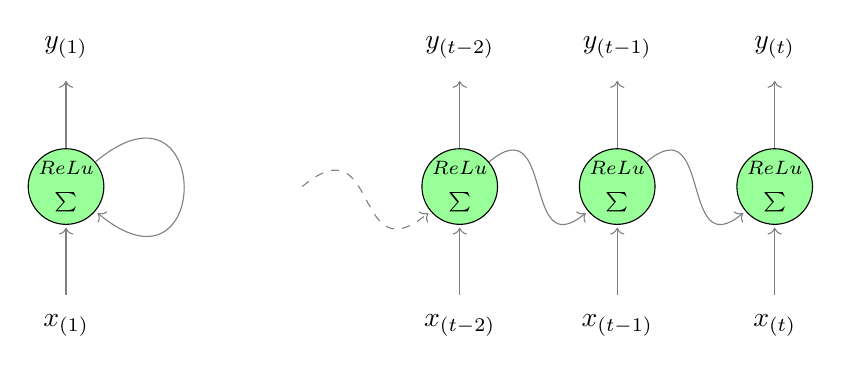
\begin{tikzpicture}[shorten >=1pt,->,draw=black!50, node distance=\layersep]
%https://tex.stackexchange.com/questions/96846/how-to-place-label-in-middle-of-line-above-and-below-with-tikz
    \tikzstyle{every pin edge}=[<-,shorten <=1pt]
    \tikzstyle{neuron}=[circle,fill=black!25,minimum size=17pt,inner sep=0pt, draw=black]
    \tikzstyle{input neuron}=[neuron, fill=green!40];
    \tikzstyle{output neuron}=[neuron, fill=red!50];
    \tikzstyle{hidden neuron}=[neuron, fill=blue!30];
    \tikzstyle{annot} = [text width=10em, text centered]


%    \node[annot,above of=H-1, node distance=1cm] (hl) {Multilabel Perceptron};

	\node[] (I) at (-3,-1.5){};
	\node[below] at (I){$x_{(1)}$};
	\node[input neuron] (R) at (-3,0) {$\substack{ReLu\\ \\\sum}$};
	\node[] (O) at (-3,1.5){};
	\node[above] at (O){$y_{(1)}$};
	\path (R) edge (O);
	\path (I) edge (R);
	\draw (R) to [out=40,in=-40,looseness=8] (R);


		 \node (I-2) at (2,-1.5){};
		 \node[input neuron] (R-2) at (2,0) {$\substack{ReLu\\ \\\sum}$};
		 \node (O-2) at (2,1.5){};
		 \node[below] at (I-2){$x_{(t-2)}$};
		 \node[above] at (O-2){$y_{(t-2)}$};
		 \path (R-2) edge (O-2);
		 \path (I-2) edge (R-2);

		 \node (I-4) at (4,-1.5){};
		 \node[input neuron] (R-4) at (4,0) {$\substack{ReLu\\ \\\sum}$};
		 \node (O-4) at (4,1.5){};
		 \node[below] at (I-4){$x_{(t-1)}$};
		 \node[above] at (O-4){$y_{(t-1)}$};
		 \path (R-4) edge (O-4);
		 \path (I-4) edge (R-4);

		 \node (I-6) at (6,-1.5){};
		 \node[input neuron] (R-6) at (6,0) {$\substack{ReLu\\ \\\sum}$};
		 \node (O-6) at (6,1.5){};
		 \node[below] at (I-6){$x_{(t)}$};
		 \node[above] at (O-6){$y_{(t)}$};
		 \path (R-6) edge (O-6);
		 \path (I-6) edge (R-6);
		 

	 \draw[dashed] (0,0) to [out=40,in=220,looseness=2] (R-2);
	 \draw (R-2) to [out=40,in=220,looseness=2] (R-4);
	 \draw (R-4) to [out=40,in=220,looseness=2] (R-6);
	
\end{tikzpicture}
  \end{minipage}
  \vfill
\begin{minipage}[t][0.5\textheight][t]{\textwidth}
Unlike feed forward networks, recurrent networks contain nodes that connect back to themselves. Looking at the simplest (one neuron) network, at each \textbf{time step} or \textbf{frame} $t$, the RNN receives inputs from $x_{(t)}$ and the previous time-step $y_{(t-1)}$.  
\end{minipage}
\end{frame}





\begin{frame}[fragile]{Recurrent Nodes}
  \begin{minipage}[t][0.5\textheight][t]{\textwidth}
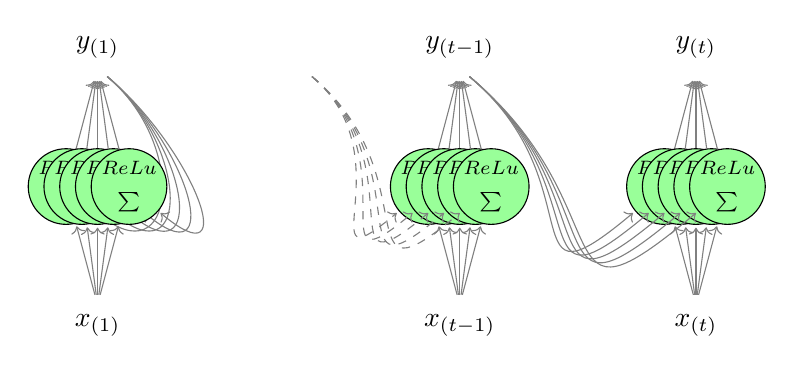
\begin{tikzpicture}[shorten >=1pt,->,draw=black!50, node distance=\layersep]
%https://tex.stackexchange.com/questions/96846/how-to-place-label-in-middle-of-line-above-and-below-with-tikz
    \tikzstyle{every pin edge}=[<-,shorten <=1pt]
    \tikzstyle{neuron}=[circle,fill=black!25,minimum size=17pt,inner sep=0pt, draw=black]
    \tikzstyle{input neuron}=[neuron, fill=green!40];
    \tikzstyle{output neuron}=[neuron, fill=red!50];
    \tikzstyle{hidden neuron}=[neuron, fill=blue!30];
    \tikzstyle{annot} = [text width=10em, text centered]


%    \node[annot,above of=H-1, node distance=1cm] (hl) {Multilabel Perceptron};


	\node[] (I) at (-2.6,-1.5){};
	\node[below] at (I){$x_{(1)}$};
	\node[] (O) at (-2.6,1.5){};
	\node[above] at (O){$y_{(1)}$};

	\foreach \x in {0,1,2,3,4}{
		\pgfmathsetmacro\y{-3+\x/5}
		\node[input neuron] (R-\x) at (\y,0) {$\substack{ReLu\\ \\\sum}$};
		\path (R-\x) edge (O);
		\path (I) edge (R-\x);
		\draw (O) to [out=-40,in=-40,looseness=2] (R-\x);
		}


	\node[] (I1) at (2,-1.5){};
	\node[below] at (I1){$x_{(t-1)}$};
	\node[] (O1) at (2,1.5){};
	\node[above] at (O1){$y_{(t-1)}$};

	\node[] (O0) at (0,1.5){};

	\foreach \x in {0,1,2,3,4}{
		\pgfmathsetmacro\y{1.6+\x/5}
		\node[input neuron] (R1-\x) at (\y,0) {$\substack{ReLu\\ \\\sum}$};
		\path (R1-\x) edge (O1);
		\path (I1) edge (R1-\x);
		\draw[dashed] (O0) to [out=-40,in=220,looseness=2] (R1-\x);
		}

	\node[] (I2) at (5,-1.5){};
	\node[below] at (I2){$x_{(t)}$};
	\node[] (O2) at (5,1.5){};
	\node[above] at (O2){$y_{(t)}$};

	\foreach \x in {0,1,2,3,4}{
		\pgfmathsetmacro\y{4.6+\x/5}
		\node[input neuron] (R2-\x) at (\y,0) {$\substack{ReLu\\ \\\sum}$};
		\path (R2-\x) edge (O2);
		\path (I2) edge (R2-\x);
		\draw (O1) to [out=-40,in=220,looseness=2] (R2-\x);
		}
		
\end{tikzpicture}
  \end{minipage}
  \vfill
\begin{minipage}[t][0.5\textheight][t]{\textwidth}
Multiple recurrent neurons can be connected together like a perceptron layer. Then each neuron has two sets of weights: $\mathbf{w}_x^i$ for the inputs $x_{(t)}$ and $\mathbf{w}_y^i$ for the outputs $y_{(t-1)}$. \pause We can collect these into matrices $\mathbf{W}_x$ and $\mathbf{W}_y$. \pause Then, for activation $\sigma$ and bias $b$, 

$$
\mathbf{Y}_{(t)} = \sigma\big( \mathbf{W}_x^T \mathbf{X}_{(t)} + \mathbf{W}_y^T \mathbf{Y}_{(t-1)} + b \big)
$$
\end{minipage}
\end{frame}









\begin{frame}[fragile]{Memory Cells}
  \begin{minipage}[t][0.5\textheight][t]{\textwidth}
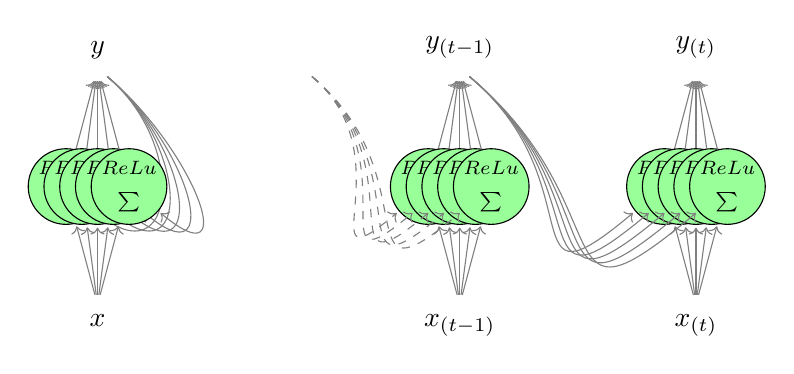
\begin{tikzpicture}[shorten >=1pt,->,draw=black!50, node distance=\layersep]
%https://tex.stackexchange.com/questions/96846/how-to-place-label-in-middle-of-line-above-and-below-with-tikz
    \tikzstyle{every pin edge}=[<-,shorten <=1pt]
    \tikzstyle{neuron}=[circle,fill=black!25,minimum size=17pt,inner sep=0pt, draw=black]
    \tikzstyle{input neuron}=[neuron, fill=green!40];
    \tikzstyle{output neuron}=[neuron, fill=red!50];
    \tikzstyle{hidden neuron}=[neuron, fill=blue!30];
    \tikzstyle{annot} = [text width=10em, text centered]


%    \node[annot,above of=H-1, node distance=1cm] (hl) {Multilabel Perceptron};


	\node[] (I) at (-2.6,-1.5){};
	\node[below] at (I){$x$};
	\node[] (O) at (-2.6,1.5){};
	\node[above] at (O){$y$};

	\foreach \x in {0,1,2,3,4}{
		\pgfmathsetmacro\y{-3+\x/5}
		\node[input neuron] (R-\x) at (\y,0) {$\substack{ReLu\\ \\\sum}$};
		\path (R-\x) edge (O);
		\path (I) edge (R-\x);
		\draw (O) to [out=-40,in=-40,looseness=2] (R-\x);
		}


	\node[] (I1) at (2,-1.5){};
	\node[below] at (I1){$x_{(t-1)}$};
	\node[] (O1) at (2,1.5){};
	\node[above] at (O1){$y_{(t-1)}$};

	\node[] (O0) at (0,1.5){};

	\foreach \x in {0,1,2,3,4}{
		\pgfmathsetmacro\y{1.6+\x/5}
		\node[input neuron] (R1-\x) at (\y,0) {$\substack{ReLu\\ \\\sum}$};
		\path (R1-\x) edge (O1);
		\path (I1) edge (R1-\x);
		\draw[dashed] (O0) to [out=-40,in=220,looseness=2] (R1-\x);
		}

	\node[] (I2) at (5,-1.5){};
	\node[below] at (I2){$x_{(t)}$};
	\node[] (O2) at (5,1.5){};
	\node[above] at (O2){$y_{(t)}$};

	\foreach \x in {0,1,2,3,4}{
		\pgfmathsetmacro\y{4.6+\x/5}
		\node[input neuron] (R2-\x) at (\y,0) {$\substack{ReLu\\ \\\sum}$};
		\path (R2-\x) edge (O2);
		\path (I2) edge (R2-\x);
		\draw (O1) to [out=-40,in=220,looseness=2] (R2-\x);
		}
		
\end{tikzpicture}
  \end{minipage}
  \vfill
\begin{minipage}[t][0.5\textheight][t]{\textwidth}
Any cell that passes information to the next frame is called a \textbf{memory cell}. In the above we pass the output of the previous frame to produce \textbf{short term memory}, but we could of course pass another state vector as well to produce \textbf{long term memory}. 
\end{minipage}
\end{frame}






\begin{frame}[fragile]{Recurrent Nodes}
  \begin{minipage}[t][0.5\textheight][t]{\textwidth}
  \begin{center}
  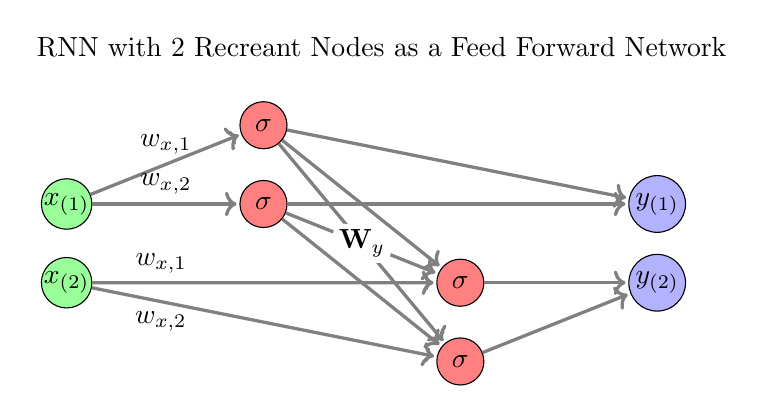
\begin{tikzpicture}[shorten >=1pt,->,draw=black!50, node distance=\layersep]
%https://tex.stackexchange.com/questions/96846/how-to-place-label-in-middle-of-line-above-and-below-with-tikz
    \tikzstyle{every pin edge}=[<-,shorten <=1pt]
    \tikzstyle{neuron}=[circle,fill=black!25,minimum size=17pt,inner sep=0pt, draw=black]
    \tikzstyle{input neuron}=[neuron, fill=green!40];
    \tikzstyle{output neuron}=[neuron, fill=red!50];
    \tikzstyle{hidden neuron}=[neuron, fill=blue!30];
    \tikzstyle{lab}=[draw=white, fill=white!80,, rectangle, rounded corners, inner sep=2pt, inner ysep=2pt]
    \tikzstyle{annot} = [text width=20em, text centered]

    % Draw the input layer nodes
	\node[input neuron] (I-1) at (0,-1) {$x_{(1)}$};
	\node[input neuron] (I-2) at (0,-2) {$x_{(2)}$};
%     \node[input neuron] (I-3) at (0,-3) {$1$};	
    % Draw the hidden layer nodes

     \node[output neuron] (H-1) at (\layersep,-0 cm) {$\,\sigma\,$};
	 \node[output neuron] (H-2) at (\layersep,- 1 cm) {$\,\sigma\,$};
	 
	 \node[output neuron] (H-3) at (\layersep+\layersep, -2 cm) {$\,\sigma\,$};
	 \node[output neuron] (H-4) at (\layersep+\layersep,- 3 cm) {$\,\sigma\,$};

	 \node[hidden neuron] (H-5) at (\layersep+\layersep+\layersep,-1 cm) {$\,y_{(1)}\,$};
	 \node[hidden neuron] (H-6) at (\layersep+\layersep+\layersep,-2 cm) {$\,y_{(2)}\,$};


	 \draw[very thick] (I-1) -- (H-1);
	 \draw[very thick] (I-1) -- (H-2);
	 \draw[very thick] (I-2) -- (H-3);
	 \draw[very thick] (I-2) -- (H-4);
	 \draw[very thick] (H-1) -- (H-5);
	 \draw[very thick] (H-2) -- (H-5);
	 \draw[very thick] (H-1) -- (H-3);
	 \draw[very thick] (H-2) -- (H-4);
	 \draw[very thick] (H-1) -- (H-4);
	 \draw[very thick] (H-2) -- (H-3);
	 \draw[very thick] (H-3) -- (H-6);
	 \draw[very thick] (H-4) -- (H-6);

	\draw (I-1) -- node[above, pos=0.5] {$w_{x,1}$} ++ (H-1);	
	\draw (I-1) -- node[below, pos=0.5] {$w_{x,2}$} ++ (H-1);	

	\draw (I-2) -- node[above, pos=0.2] {$w_{x,1}$} ++ (H-3);
	\draw (I-2) -- node[below, pos=0.2] {$w_{x,2}$} ++ (H-4);

	\draw (H-1) -- node[lab, pos=0.5] {$\mathbf{W}_{y}$} ++ (H-4);

    \node at (4cm ,1cm) {RNN with 2 Recreant Nodes as a Feed Forward Network};
\end{tikzpicture}
\end{center}
  \end{minipage}
  \vfill
\begin{minipage}[t][0.5\textheight][t]{\textwidth}
We can represent the node function
$$
\mathbf{Y}_{(t)} = \sigma\big( \mathbf{W}_x^T \mathbf{X}_{(t)} + \mathbf{W}_y^T \mathbf{Y}_{(t-1)} + b \big)
$$
as a feed forward network. However, we immediately see that this network will get very deep fast. In addition, since $\mathbf{Y}_{(t)}$ depends on $\mathbf{Y}_{(t-1)}$, this will be a highly nonlinear function of $\mathbf{W}_y^T $.
\end{minipage}
\end{frame}





\begin{frame}[fragile]{Recurrent Nodes}
  \begin{minipage}[t][0.5\textheight][t]{\textwidth}
  \begin{center}
  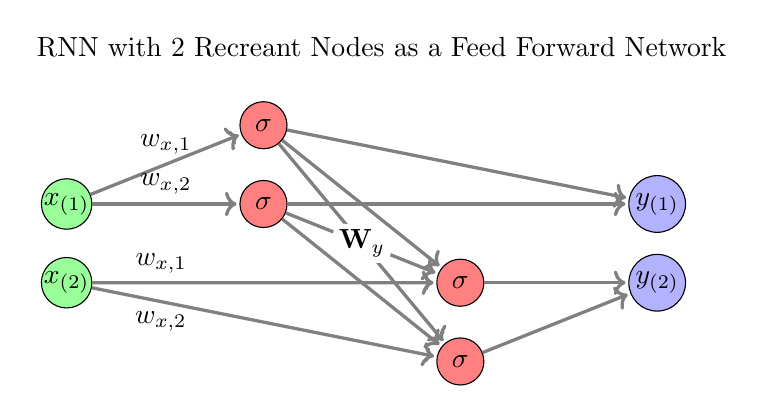
\begin{tikzpicture}[shorten >=1pt,->,draw=black!50, node distance=\layersep]
%https://tex.stackexchange.com/questions/96846/how-to-place-label-in-middle-of-line-above-and-below-with-tikz
    \tikzstyle{every pin edge}=[<-,shorten <=1pt]
    \tikzstyle{neuron}=[circle,fill=black!25,minimum size=17pt,inner sep=0pt, draw=black]
    \tikzstyle{input neuron}=[neuron, fill=green!40];
    \tikzstyle{output neuron}=[neuron, fill=red!50];
    \tikzstyle{hidden neuron}=[neuron, fill=blue!30];
    \tikzstyle{lab}=[draw=white, fill=white!80,, rectangle, rounded corners, inner sep=2pt, inner ysep=2pt]
    \tikzstyle{annot} = [text width=20em, text centered]

    % Draw the input layer nodes
	\node[input neuron] (I-1) at (0,-1) {$x_{(1)}$};
	\node[input neuron] (I-2) at (0,-2) {$x_{(2)}$};
%     \node[input neuron] (I-3) at (0,-3) {$1$};	
    % Draw the hidden layer nodes

     \node[output neuron] (H-1) at (\layersep,-0 cm) {$\,\sigma\,$};
	 \node[output neuron] (H-2) at (\layersep,- 1 cm) {$\,\sigma\,$};
	 
	 \node[output neuron] (H-3) at (\layersep+\layersep, -2 cm) {$\,\sigma\,$};
	 \node[output neuron] (H-4) at (\layersep+\layersep,- 3 cm) {$\,\sigma\,$};

	 \node[hidden neuron] (H-5) at (\layersep+\layersep+\layersep,-1 cm) {$\,y_{(1)}\,$};
	 \node[hidden neuron] (H-6) at (\layersep+\layersep+\layersep,-2 cm) {$\,y_{(2)}\,$};


	 \draw[very thick] (I-1) -- (H-1);
	 \draw[very thick] (I-1) -- (H-2);
	 \draw[very thick] (I-2) -- (H-3);
	 \draw[very thick] (I-2) -- (H-4);
	 \draw[very thick] (H-1) -- (H-5);
	 \draw[very thick] (H-2) -- (H-5);
	 \draw[very thick] (H-1) -- (H-3);
	 \draw[very thick] (H-2) -- (H-4);
	 \draw[very thick] (H-1) -- (H-4);
	 \draw[very thick] (H-2) -- (H-3);
	 \draw[very thick] (H-3) -- (H-6);
	 \draw[very thick] (H-4) -- (H-6);

	\draw (I-1) -- node[above, pos=0.5] {$w_{x,1}$} ++ (H-1);	
	\draw (I-1) -- node[below, pos=0.5] {$w_{x,2}$} ++ (H-1);	

	\draw (I-2) -- node[above, pos=0.2] {$w_{x,1}$} ++ (H-3);
	\draw (I-2) -- node[below, pos=0.2] {$w_{x,2}$} ++ (H-4);

	\draw (H-1) -- node[lab, pos=0.5] {$\mathbf{W}_{y}$} ++ (H-4);

    \node at (4cm ,1cm) {RNN with 2 Recreant Nodes as a Feed Forward Network};
\end{tikzpicture}
\end{center}
  \end{minipage}
  \vfill
\begin{minipage}[t][0.5\textheight][t]{\textwidth}
However this also gives a straightforward way to train the network: we simply unroll it into a feed forward network and train it with back propagation. Notice as well that since the weights are shared between recurrent nodes we can unroll network to any depth we want. In principle, we could train on short sequences and then use the network to predict long sequences. Practically, this means the same RNN can be used for many different tasks. 
\end{minipage}
\end{frame}















\begin{frame}[fragile]{Basic RNN Structures}
  \begin{minipage}[t][0.5\textheight][t]{\textwidth}\centering
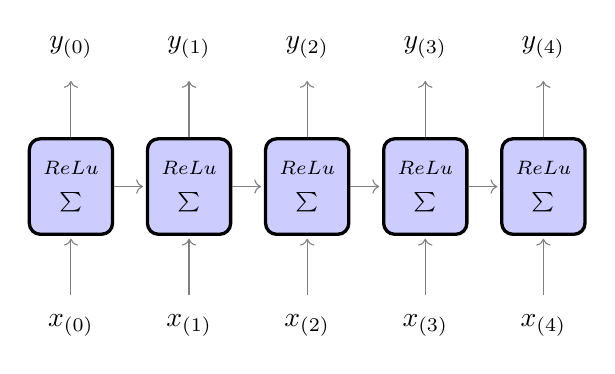
\begin{tikzpicture}[shorten >=1pt,->,draw=black!50, node distance=\layersep]
%https://tex.stackexchange.com/questions/96846/how-to-place-label-in-middle-of-line-above-and-below-with-tikz
    \tikzstyle{every pin edge}=[<-,shorten <=1pt]
    \tikzstyle{neuron}=[circle,fill=black!25,minimum size=17pt,inner sep=0pt, draw=black]
    \tikzstyle{layer}=[draw=black, fill=blue!20, very thick, rectangle, rounded corners, inner sep=5pt, inner ysep=8pt]
    \tikzstyle{input neuron}=[neuron, fill=green!40];
    \tikzstyle{output neuron}=[neuron, fill=red!50];
    \tikzstyle{hidden neuron}=[neuron, fill=blue!30];
    \tikzstyle{annot} = [text width=10em, text centered]


%    \node[annot,above of=H-1, node distance=1cm] (hl) {Multilabel Perceptron};


	\foreach \x in {0,1,2,3,4}{
		\pgfmathsetmacro\y{-3+\x*1.5}
		\node[] (I-\x) at (\y,-1.5){};
		\node[below] at (I-\x){$x_{(\x)}$};
		\node[] (O-\x) at (\y,1.5){};
		\node[above] at (O-\x){$y_{(\x)}$};
		\node[layer] (R-\x) at (\y,0) {$\substack{ReLu\\ \\\sum}$};
		\path (I-\x) edge (R-\x);
		\path (R-\x) edge (O-\x);
	}

		\path (R-0) edge (R-1);
		\path (R-1) edge (R-2);
		\path (R-2) edge (R-3);
		\path (R-3) edge (R-4);
\end{tikzpicture}
  \end{minipage}
  \vfill
\begin{minipage}[t][0.5\textheight][t]{\textwidth}
A RNN can take in a series of inputs and produce a series of outputs, as in predicting time series data like stock prices or traffic across a network. 
\end{minipage}
\end{frame}



\begin{frame}[fragile]{Basic RNN Structures}
  \begin{minipage}[t][0.5\textheight][t]{\textwidth}\centering
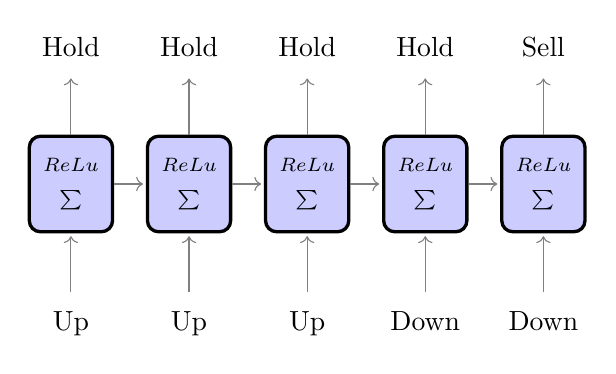
\begin{tikzpicture}[shorten >=1pt,->,draw=black!50, node distance=\layersep]
%https://tex.stackexchange.com/questions/96846/how-to-place-label-in-middle-of-line-above-and-below-with-tikz
    \tikzstyle{every pin edge}=[<-,shorten <=1pt]
    \tikzstyle{neuron}=[circle,fill=black!25,minimum size=17pt,inner sep=0pt, draw=black]
    \tikzstyle{layer}=[draw=black, fill=blue!20, very thick, rectangle, rounded corners, inner sep=5pt, inner ysep=8pt]
    \tikzstyle{input neuron}=[neuron, fill=green!40];
    \tikzstyle{output neuron}=[neuron, fill=red!50];
    \tikzstyle{hidden neuron}=[neuron, fill=blue!30];
    \tikzstyle{annot} = [text width=10em, text centered]


%    \node[annot,above of=H-1, node distance=1cm] (hl) {Multilabel Perceptron};


	\foreach \x in {0,1,2}{
		\pgfmathsetmacro\y{-3+\x*1.5}
		\node[] (I-\x) at (\y,-1.5){};
		\node[below] at (I-\x){Up};
		\node[] (O-\x) at (\y,1.5){};
		\node[above] at (O-\x){Hold};
		\node[layer] (R-\x) at (\y,0) {$\substack{ReLu\\ \\\sum}$};
		\path (I-\x) edge (R-\x);
		\path (R-\x) edge (O-\x);
	}
	
	\foreach \x in {3}{
		\pgfmathsetmacro\y{-3+\x*1.5}
		\node[] (I-\x) at (\y,-1.5){};
		\node[below] at (I-\x){Down};
		\node[] (O-\x) at (\y,1.5){};
		\node[above] at (O-\x){Hold};
		\node[layer] (R-\x) at (\y,0) {$\substack{ReLu\\ \\\sum}$};
		\path (I-\x) edge (R-\x);
		\path (R-\x) edge (O-\x);
	}	
	
	\foreach \x in {4}{
		\pgfmathsetmacro\y{-3+\x*1.5}
		\node[] (I-\x) at (\y,-1.5){};
		\node[below] at (I-\x){Down};
		\node[] (O-\x) at (\y,1.5){};
		\node[above] at (O-\x){Sell};
		\node[layer] (R-\x) at (\y,0) {$\substack{ReLu\\ \\\sum}$};
		\path (I-\x) edge (R-\x);
		\path (R-\x) edge (O-\x);
	}

		\path (R-0) edge (R-1);
		\path (R-1) edge (R-2);
		\path (R-2) edge (R-3);
		\path (R-3) edge (R-4);
\end{tikzpicture}
  \end{minipage}
  \vfill
\begin{minipage}[t][0.5\textheight][t]{\textwidth}
A RNN can take in a series of inputs and produce a series of outputs, as in predicting time series data like stock prices or traffic across a network. 
\end{minipage}
\end{frame}






\begin{frame}[fragile]{Basic RNN Structures}
  \begin{minipage}[t][0.5\textheight][t]{\textwidth}\centering
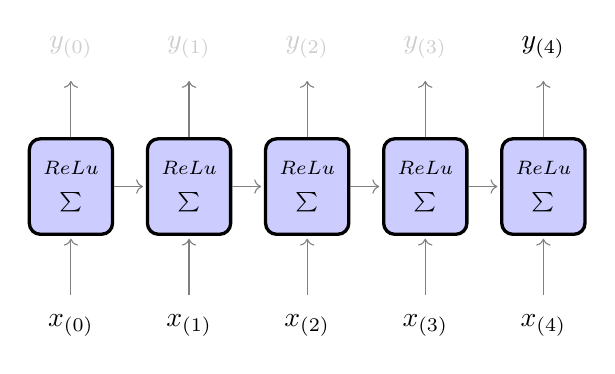
\begin{tikzpicture}[shorten >=1pt,->,draw=black!50, node distance=\layersep]
%https://tex.stackexchange.com/questions/96846/how-to-place-label-in-middle-of-line-above-and-below-with-tikz
    \tikzstyle{every pin edge}=[<-,shorten <=1pt]
    \tikzstyle{neuron}=[circle,fill=black!25,minimum size=17pt,inner sep=0pt, draw=black]
    \tikzstyle{layer}=[draw=black, fill=blue!20, very thick, rectangle, rounded corners, inner sep=5pt, inner ysep=8pt]
    \tikzstyle{input neuron}=[neuron, fill=green!40];
    \tikzstyle{output neuron}=[neuron, fill=red!50];
    \tikzstyle{hidden neuron}=[neuron, fill=blue!30];
    \tikzstyle{annot} = [text width=10em, text centered]


%    \node[annot,above of=H-1, node distance=1cm] (hl) {Multilabel Perceptron};


	\foreach \x in {0,1,2,3,4}{
		\pgfmathsetmacro\y{-3+\x*1.5}
		\node[] (I-\x) at (\y,-1.5){};
		\node[below] at (I-\x){$x_{(\x)}$};
		\node[] (O-\x) at (\y,1.5){};
		\node[above, opacity=.2] at (O-\x){$y_{(\x)}$};
		\node[layer] (R-\x) at (\y,0) {$\substack{ReLu\\ \\\sum}$};
		\path (I-\x) edge (R-\x);
		\path (R-\x) edge (O-\x);
	}

	\node[above] at (O-4){$y_{(4)}$};

	\path (R-0) edge (R-1);
	\path (R-1) edge (R-2);
	\path (R-2) edge (R-3);
	\path (R-3) edge (R-4);
\end{tikzpicture}
  \end{minipage}
  \vfill
\begin{minipage}[t][0.5\textheight][t]{\textwidth}
Alternatively, you can feed in many inputs but only record the last output, like in text prediction. 
\end{minipage}
\end{frame}




\begin{frame}[fragile]{Basic RNN Structures}
  \begin{minipage}[t][0.5\textheight][t]{\textwidth}\centering
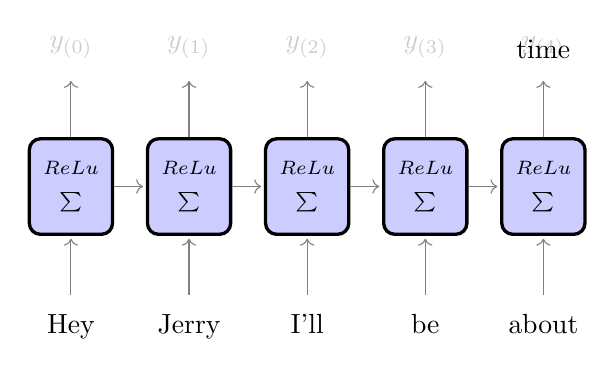
\begin{tikzpicture}[shorten >=1pt,->,draw=black!50, node distance=\layersep]
%https://tex.stackexchange.com/questions/96846/how-to-place-label-in-middle-of-line-above-and-below-with-tikz
    \tikzstyle{every pin edge}=[<-,shorten <=1pt]
    \tikzstyle{neuron}=[circle,fill=black!25,minimum size=17pt,inner sep=0pt, draw=black]
    \tikzstyle{layer}=[draw=black, fill=blue!20, very thick, rectangle, rounded corners, inner sep=5pt, inner ysep=8pt]
    \tikzstyle{input neuron}=[neuron, fill=green!40];
    \tikzstyle{output neuron}=[neuron, fill=red!50];
    \tikzstyle{hidden neuron}=[neuron, fill=blue!30];
    \tikzstyle{annot} = [text width=10em, text centered]


%    \node[annot,above of=H-1, node distance=1cm] (hl) {Multilabel Perceptron};


	\foreach \x in {0,1,2,3,4}{
		\pgfmathsetmacro\y{-3+\x*1.5}
		\node[] (I-\x) at (\y,-1.5){};
		\node[] (O-\x) at (\y,1.5){};
		\node[above, opacity=.2] at (O-\x){$y_{(\x)}$};
		\node[layer] (R-\x) at (\y,0) {$\substack{ReLu\\ \\\sum}$};
		\path (I-\x) edge (R-\x);
		\path (R-\x) edge (O-\x);
	}
	\node[below] at (I-0){Hey};
	\node[below] at (I-1){Jerry};
	\node[below] at (I-2){I'll};
	\node[below] at (I-3){be};
	\node[below] at (I-4){about};
	\node[above] at (O-4){time};

	\path (R-0) edge (R-1);
	\path (R-1) edge (R-2);
	\path (R-2) edge (R-3);
	\path (R-3) edge (R-4);
\end{tikzpicture}
  \end{minipage}
  \vfill
\begin{minipage}[t][0.5\textheight][t]{\textwidth}
Alternatively, you can feed in many inputs but only record the last output, like in text prediction. 
\end{minipage}
\end{frame}






\begin{frame}[fragile]{Basic RNN Structures}
  \begin{minipage}[t][0.5\textheight][t]{\textwidth}\centering
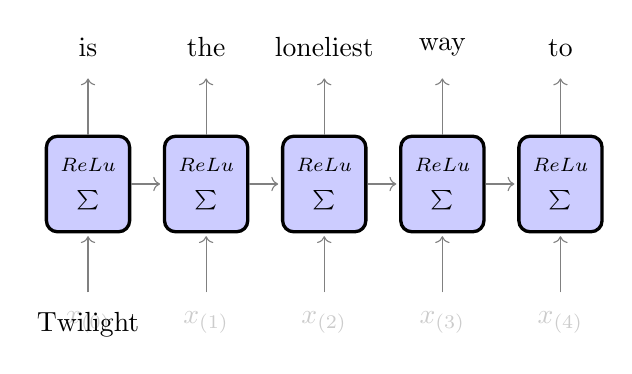
\begin{tikzpicture}[shorten >=1pt,->,draw=black!50, node distance=\layersep]
%https://tex.stackexchange.com/questions/96846/how-to-place-label-in-middle-of-line-above-and-below-with-tikz
    \tikzstyle{every pin edge}=[<-,shorten <=1pt]
    \tikzstyle{neuron}=[circle,fill=black!25,minimum size=17pt,inner sep=0pt, draw=black]
    \tikzstyle{layer}=[draw=black, fill=blue!20, very thick, rectangle, rounded corners, inner sep=5pt, inner ysep=8pt]
    \tikzstyle{input neuron}=[neuron, fill=green!40];
    \tikzstyle{output neuron}=[neuron, fill=red!50];
    \tikzstyle{hidden neuron}=[neuron, fill=blue!30];
    \tikzstyle{annot} = [text width=10em, text centered]


%    \node[annot,above of=H-1, node distance=1cm] (hl) {Multilabel Perceptron};


	\foreach \x in {0,1,2,3,4}{
		\pgfmathsetmacro\y{-3+\x*1.5}
		\node[] (I-\x) at (\y,-1.5){};
		\node[below, opacity=.2] at (I-\x){$x_{(\x)}$};
		\node[] (O-\x) at (\y,1.5){};
%		\node[above] at (O-\x){$y_{(\x)}$};
		\node[layer] (R-\x) at (\y,0) {$\substack{ReLu\\ \\\sum}$};
		\path (I-\x) edge (R-\x);
		\path (R-\x) edge (O-\x);
	}

	\node[below] at (I-0){Twilight};
	\node[above] at (O-0){is};
	\node[above] at (O-1){the};
	\node[above] at (O-2){loneliest};
	\node[above] at (O-3){way};
	\node[above] at (O-4){to};

	\path (R-0) edge (R-1);
	\path (R-1) edge (R-2);
	\path (R-2) edge (R-3);
	\path (R-3) edge (R-4);
\end{tikzpicture}
  \end{minipage}
  \vfill
\begin{minipage}[t][0.5\textheight][t]{\textwidth}
We can also use a trained RNN to predict a sequence of data by only priming on a single (or a small number) of time steps and then outputting a series data based on that input. This is one way to produce generative networks. 
\end{minipage}
\end{frame}





\begin{frame}[fragile]{Basic RNN Structures}
  \begin{minipage}[t][0.5\textheight][t]{\textwidth}\centering
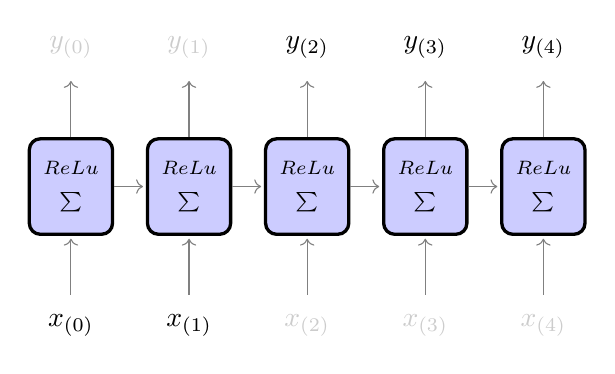
\begin{tikzpicture}[shorten >=1pt,->,draw=black!50, node distance=\layersep]
%https://tex.stackexchange.com/questions/96846/how-to-place-label-in-middle-of-line-above-and-below-with-tikz
    \tikzstyle{every pin edge}=[<-,shorten <=1pt]
    \tikzstyle{neuron}=[circle,fill=black!25,minimum size=17pt,inner sep=0pt, draw=black]
    \tikzstyle{layer}=[draw=black, fill=blue!20, very thick, rectangle, rounded corners, inner sep=5pt, inner ysep=8pt]
    \tikzstyle{input neuron}=[neuron, fill=green!40];
    \tikzstyle{output neuron}=[neuron, fill=red!50];
    \tikzstyle{hidden neuron}=[neuron, fill=blue!30];
    \tikzstyle{annot} = [text width=10em, text centered]


%    \node[annot,above of=H-1, node distance=1cm] (hl) {Multilabel Perceptron};


	\foreach \x in {0,1,2,3,4}{
		\pgfmathsetmacro\y{-3+\x*1.5}
		\node[] (I-\x) at (\y,-1.5){};
		\node[below, opacity=.2] at (I-\x){$x_{(\x)}$};
		\node[] (O-\x) at (\y,1.5){};
		\node[above, opacity=.2] at (O-\x){$y_{(\x)}$};
		\node[layer] (R-\x) at (\y,0) {$\substack{ReLu\\ \\\sum}$};
		\path (I-\x) edge (R-\x);
		\path (R-\x) edge (O-\x);
	}

	\node[below] at (I-0){$x_{(0)}$};
	\node[below] at (I-1){$x_{(1)}$};
	\node[above] at (O-2){$y_{(2)}$};
	\node[above] at (O-3){$y_{(3)}$};
	\node[above] at (O-4){$y_{(4)}$};

	\path (R-0) edge (R-1);
	\path (R-1) edge (R-2);
	\path (R-2) edge (R-3);
	\path (R-3) edge (R-4);
\end{tikzpicture}
  \end{minipage}
  \vfill
\begin{minipage}[t][0.5\textheight][t]{\textwidth}
Finally, we can consider encoder/decoder networks where we feed in data encoding it, use the RNN to process it, and then return a new sequence. For example in a translation RNN you would feed $n$ words into the network and return a sentence of an arbitrary length. \pause  In such a situation, you should train an "end of sentence" character to signify when the network should stop. 
\end{minipage}
\end{frame}







\begin{frame}[fragile]{Basic RNN Structures}
  \begin{minipage}[t][0.5\textheight][t]{\textwidth}\centering
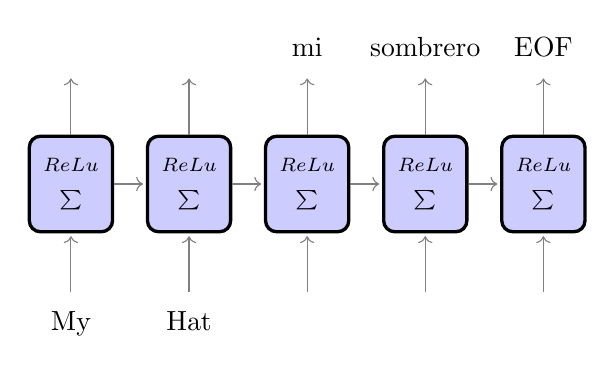
\begin{tikzpicture}[shorten >=1pt,->,draw=black!50, node distance=\layersep]
%https://tex.stackexchange.com/questions/96846/how-to-place-label-in-middle-of-line-above-and-below-with-tikz
    \tikzstyle{every pin edge}=[<-,shorten <=1pt]
    \tikzstyle{neuron}=[circle,fill=black!25,minimum size=17pt,inner sep=0pt, draw=black]
    \tikzstyle{layer}=[draw=black, fill=blue!20, very thick, rectangle, rounded corners, inner sep=5pt, inner ysep=8pt]
    \tikzstyle{input neuron}=[neuron, fill=green!40];
    \tikzstyle{output neuron}=[neuron, fill=red!50];
    \tikzstyle{hidden neuron}=[neuron, fill=blue!30];
    \tikzstyle{annot} = [text width=10em, text centered]


%    \node[annot,above of=H-1, node distance=1cm] (hl) {Multilabel Perceptron};


	\foreach \x in {0,1,2,3,4}{
		\pgfmathsetmacro\y{-3+\x*1.5}
		\node[] (I-\x) at (\y,-1.5){};
%		\node[below, opacity=.2] at (I-\x){$x_{(\x)}$};
		\node[] (O-\x) at (\y,1.5){};
%		\node[above, opacity=.2] at (O-\x){$y_{(\x)}$};
		\node[layer] (R-\x) at (\y,0) {$\substack{ReLu\\ \\\sum}$};
		\path (I-\x) edge (R-\x);
		\path (R-\x) edge (O-\x);
	}

	\node[below] at (I-0){My};
	\node[below] at (I-1){Hat};
	\node[above] at (O-2){mi};
	\node[above] at (O-3){sombrero};
	\node[above] at (O-4){EOF};

	\path (R-0) edge (R-1);
	\path (R-1) edge (R-2);
	\path (R-2) edge (R-3);
	\path (R-3) edge (R-4);
\end{tikzpicture}
  \end{minipage}
  \vfill
\begin{minipage}[t][0.5\textheight][t]{\textwidth}
Finally, we can consider encoder/decoder networks where we feed in data encoding it, use the RNN to process it, and then return a new sequence. For example in a translation RNN you would feed $n$ words into the network and return a sentence of an arbitrary length. \pause  In such a situation, you should train an "end of sentence" character to signify when the network should stop. 
\end{minipage}
\end{frame}





\begin{frame}[fragile]{Training: Backpropagation}
  \begin{minipage}[t][0.5\textheight][t]{\textwidth}\centering
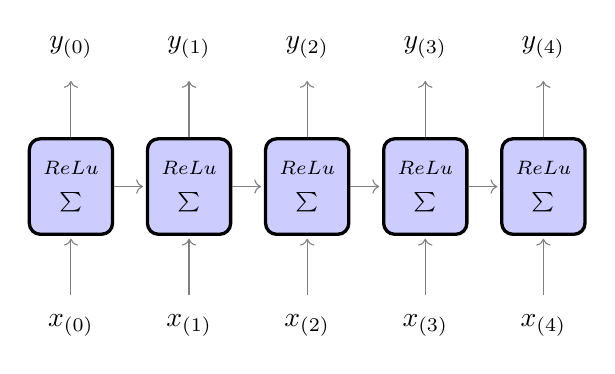
\begin{tikzpicture}[shorten >=1pt,->,draw=black!50, node distance=\layersep]
%https://tex.stackexchange.com/questions/96846/how-to-place-label-in-middle-of-line-above-and-below-with-tikz
    \tikzstyle{every pin edge}=[<-,shorten <=1pt]
    \tikzstyle{neuron}=[circle,fill=black!25,minimum size=17pt,inner sep=0pt, draw=black]
    \tikzstyle{layer}=[draw=black, fill=blue!20, very thick, rectangle, rounded corners, inner sep=5pt, inner ysep=8pt]
    \tikzstyle{input neuron}=[neuron, fill=green!40];
    \tikzstyle{output neuron}=[neuron, fill=red!50];
    \tikzstyle{hidden neuron}=[neuron, fill=blue!30];
    \tikzstyle{annot} = [text width=10em, text centered]


%    \node[annot,above of=H-1, node distance=1cm] (hl) {Multilabel Perceptron};


	\foreach \x in {0,1,2,3,4}{
		\pgfmathsetmacro\y{-3+\x*1.5}
		\node[] (I-\x) at (\y,-1.5){};
		\node[below] at (I-\x){$x_{(\x)}$};
		\node[] (O-\x) at (\y,1.5){};
		\node[above] at (O-\x){$y_{(\x)}$};
		\node[layer] (R-\x) at (\y,0) {$\substack{ReLu\\ \\\sum}$};
		\path (I-\x) edge (R-\x);
		\path (R-\x) edge (O-\x);
	}

		\path (R-0) edge (R-1);
		\path (R-1) edge (R-2);
		\path (R-2) edge (R-3);
		\path (R-3) edge (R-4);
\end{tikzpicture}
  \end{minipage}
  \vfill
\begin{minipage}[t][0.5\textheight][t]{\textwidth}
To train an RNN, we unroll it to the the number of steps we require to match out input data shape and then perform standard autodiff backpropagation with input vector $\mathbf{X} = (x_{(0)},x_{(1)},\ldots, x_{(N)})$ and output $\mathbf{Y} = (y_{(0)},y_{(1)},\ldots, y_{(M)})$. \pause\newline

Note that we must define an appropriate cost function on $\mathbf{Y}$.
\end{minipage}
\end{frame}




\begin{frame}[fragile]{Example: MNIST}
  \begin{minipage}[t][0.5\textheight][t]{\textwidth}\centering
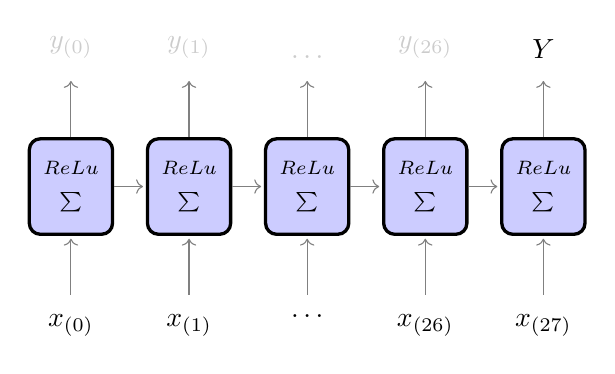
\begin{tikzpicture}[shorten >=1pt,->,draw=black!50, node distance=\layersep]
%https://tex.stackexchange.com/questions/96846/how-to-place-label-in-middle-of-line-above-and-below-with-tikz
    \tikzstyle{every pin edge}=[<-,shorten <=1pt]
    \tikzstyle{neuron}=[circle,fill=black!25,minimum size=17pt,inner sep=0pt, draw=black]
    \tikzstyle{layer}=[draw=black, fill=blue!20, very thick, rectangle, rounded corners, inner sep=5pt, inner ysep=8pt]
    \tikzstyle{input neuron}=[neuron, fill=green!40];
    \tikzstyle{output neuron}=[neuron, fill=red!50];
    \tikzstyle{hidden neuron}=[neuron, fill=blue!30];
    \tikzstyle{annot} = [text width=10em, text centered]


%    \node[annot,above of=H-1, node distance=1cm] (hl) {Multilabel Perceptron};


	\foreach \x in {0,1,2,3,4}{
		\pgfmathsetmacro\y{-3+\x*1.5}
		\node[] (I-\x) at (\y,-1.5){};
%		\node[below] at (I-\x){$x_{(\x)}$};
		\node[] (O-\x) at (\y,1.5){};
%		\node[above, opacity=.2] at (O-\x){$y_{(\x)}$};
		\node[layer] (R-\x) at (\y,0) {$\substack{ReLu\\ \\\sum}$};
		\path (I-\x) edge (R-\x);
		\path (R-\x) edge (O-\x);
	}


	\node[below] at (I-0){$x_{(0)}$};
	\node[below] at (I-1){$x_{(1)}$};
	\node[below] at (I-2){$\ldots$};
	\node[below] at (I-3){$x_{(26)}$};
	\node[below] at (I-4){$x_{(27)}$};
	\node[above, opacity=.2] at (O-0){$y_{(0)}$};
	\node[above, opacity=.2] at (O-1){$y_{(1)}$};
	\node[above, opacity=.2] at (O-2){$\ldots$};
	\node[above, opacity=.2] at (O-3){$y_{(26)}$};
	\node[above] at (O-4){$Y$};

	\path (R-0) edge (R-1);
	\path (R-1) edge (R-2);
	\path (R-2) edge (R-3);
	\path (R-3) edge (R-4);
\end{tikzpicture}
  \end{minipage}
  \vfill
\begin{minipage}[t][0.5\textheight][t]{\textwidth}
For example, we could classify $28\times 28$ MNIST using an RNN: 

\begin{itemize}
\item[] Feed each row in as a sequential vector.
\item[] Output $Y$ into a 10 node dense layer
\item[] Output to a softmax layer with 0-1 loss. 
\end{itemize}
\end{minipage}
\end{frame}


\begin{frame}[fragile]{Example: MNIST}
  \begin{minipage}[t][0.5\textheight][t]{\textwidth}\centering
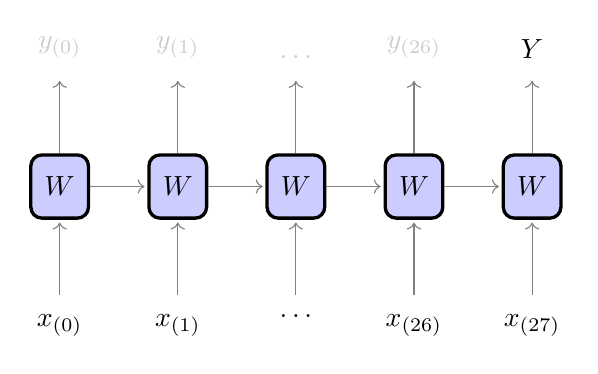
\begin{tikzpicture}[shorten >=1pt,->,draw=black!50, node distance=\layersep]
%https://tex.stackexchange.com/questions/96846/how-to-place-label-in-middle-of-line-above-and-below-with-tikz
    \tikzstyle{every pin edge}=[<-,shorten <=1pt]
    \tikzstyle{neuron}=[circle,fill=black!25,minimum size=17pt,inner sep=0pt, draw=black]
    \tikzstyle{layer}=[draw=black, fill=blue!20, very thick, rectangle, rounded corners, inner sep=5pt, inner ysep=8pt]
    \tikzstyle{input neuron}=[neuron, fill=green!40];
    \tikzstyle{output neuron}=[neuron, fill=red!50];
    \tikzstyle{hidden neuron}=[neuron, fill=blue!30];
    \tikzstyle{annot} = [text width=10em, text centered]


%    \node[annot,above of=H-1, node distance=1cm] (hl) {Multilabel Perceptron};


	\foreach \x in {0,1,2,3,4}{
		\pgfmathsetmacro\y{-3+\x*1.5}
		\node[] (I-\x) at (\y,-1.5){};
%		\node[below] at (I-\x){$x_{(\x)}$};
		\node[] (O-\x) at (\y,1.5){};
%		\node[above, opacity=.2] at (O-\x){$y_{(\x)}$};
		\node[layer] (R-\x) at (\y,0) {$W$};
		\path (I-\x) edge (R-\x);
		\path (R-\x) edge (O-\x);
	}


	\node[below] at (I-0){$x_{(0)}$};
	\node[below] at (I-1){$x_{(1)}$};
	\node[below] at (I-2){$\ldots$};
	\node[below] at (I-3){$x_{(26)}$};
	\node[below] at (I-4){$x_{(27)}$};
	\node[above, opacity=.2] at (O-0){$y_{(0)}$};
	\node[above, opacity=.2] at (O-1){$y_{(1)}$};
	\node[above, opacity=.2] at (O-2){$\ldots$};
	\node[above, opacity=.2] at (O-3){$y_{(26)}$};
	\node[above] at (O-4){$Y$};

	\path (R-0) edge (R-1);
	\path (R-1) edge (R-2);
	\path (R-2) edge (R-3);
	\path (R-3) edge (R-4);
\end{tikzpicture}
  \end{minipage}
  \vfill
\begin{minipage}[t][0.5\textheight][t]{\textwidth}
It should be noted that unrolling can be statically or dynamically implemented. Since each sequential layer in the unrolling \emph{contains a copy of the same weights} we can train and test on data with variable lengths. \pause\newline

For example, if we feed a sentence in word by word, we can unroll the RNN to be as long as we need for each sentence, since we only have a single set of weights $\mathbf{W}$ that is shared across all unrolled nodes. 
\end{minipage}
\end{frame}



\begin{frame}[fragile]{Example: Time Series}
  \begin{minipage}[t][0.5\textheight][t]{\textwidth}
	\centering \includegraphics[height=0.5\textheight]{L12Sequ.png} 
  \end{minipage}
  \vfill
\begin{minipage}[t][0.5\textheight][t]{\textwidth}
For a standard example, assume we want to predict a time series. To train, we take sequences of 40 data points from the training data and return the data shifted by 1, with a single prediction at the end. 
\end{minipage}
\end{frame}



\begin{frame}[fragile]{Example: Time Series}
  \begin{minipage}[t][0.5\textheight][t]{\textwidth}
	\centering \includegraphics[height=0.5\textheight]{L12Sequ.png} 
  \end{minipage}
  \vfill
\begin{minipage}[t][0.5\textheight][t]{\textwidth}
As an RNN then, we define a recurrence layer:
\begin{itemize}
\item[] 1 input node
\item[] 100 node dense layer
\item[] 1 output node. 
\end{itemize}\pause
and unroll it over 40 (number of points in our training instance) steps.
\end{minipage}
\end{frame}



\begin{frame}[fragile]{Example: Time Series}
  \begin{minipage}[t][0.5\textheight][t]{\textwidth}
	\centering \includegraphics[height=0.5\textheight]{L12Sequ.png} 
  \end{minipage}
  \vfill
\begin{minipage}[t][0.5\textheight][t]{\textwidth}
However, the advantage comes to the use time: Even though we have trained on sequences of 40 points, we can use the network to predict using any length of sequence. Of course, the mantra of machine learning is ``Always train on the data you will be testing on.'' For this reason, RNN's can also be constructed to require input of a specific length. 
\end{minipage}
\end{frame}




\section{Recurrence Nodes}



\begin{frame}[fragile]{LSTM Cell}
The main challenge with RNN's is that training is highly susceptible to gradient explosion and vanishing. This is thought to be because recurrent nodes lead to highly nonlinear networks, which in tern lead to gradient volatility. \pause\newline

The other challenge is training long term memory vs short term memory. If our time series network only knows about the last 40 data points it might miss long terms moves in the data. \pause\newline

One solution is to build new recurrent nodes by replace the function 
$$
\mathbf{Y}_{(t)} = \sigma\big( \mathbf{W}_x^T \mathbf{X}_{(t)} + \mathbf{W}_y^T \mathbf{Y}_{(t-1)} + b \big)
$$
with a new function tries to solve both these problems. We will finish this lecture by taking a quick look at two such example. 
\end{frame}


\begin{frame}[fragile]{LSTM Cell}
  \begin{minipage}[t][0.5\textheight][t]{\textwidth}
	\centering \includegraphics[width=0.9\textwidth]{L12LSTMOpen.png} 
  \end{minipage}
  \vfill
\begin{minipage}[t][0.5\textheight][t]{\textwidth}
The first example is a \textbf{long short-term memory} (\textbf{LSTM}) cell. At its boundary, the LSTM cell looks exactly like the recurrence cell from before, except that it sends both its output $y_{(t)}$ and a state vector $C_{(t)}$ to the next training frame. 

\url{https://colah.github.io/posts/2015-08-Understanding-LSTMs/}
\end{minipage}
\end{frame}


\begin{frame}[fragile]{LSTM Cell}
  \begin{minipage}[t][0.5\textheight][t]{\textwidth}
	\centering \includegraphics[width=0.9\textwidth]{L12LSTMOpen.png} 
  \end{minipage}
  \vfill
\begin{minipage}[t][0.5\textheight][t]{\textwidth}
In the diagram above, the product and sum are the component wise product and sum,  so at the product node $[1,2] \otimes [3,4] = [3,8]$.

\begin{center}
\includegraphics[width=0.8\textwidth]{L12LSTM2-notation.png} 
\end{center}

\end{minipage}
\end{frame}





\begin{frame}[fragile]{LSTM Cell}
  \begin{minipage}[t][0.5\textheight][t]{\textwidth}
	\centering \includegraphics[height=0.5\textheight]{L12LSTMSingle.png} 
  \end{minipage}
  \vfill
\begin{minipage}[t][0.5\textheight][t]{\textwidth}
In the LSTM node, each box represents a different LTU with the given activation function:
$$
\sigma(\mathbf{W}_x^T\mathbf{X}_t +\mathbf{W}_y^T\mathbf{h}_{t-1} +b)\,,\,\,\,\text{or}\,\,\,\text{tanh}(\mathbf{W}_x^T\mathbf{X}_t +\mathbf{W}_y^T\mathbf{h}_{t-1} +b)\,.
$$\pause
Here $\sigma$ is the sigmoid function, so the output is a vector where each element is between 0 and 1. This means that each $\sigma \otimes$ layer acts as a multiplicative mask of the connecting vector. 
\end{minipage}
\end{frame}











\begin{frame}[fragile]{LSTM Cell}
  \begin{minipage}[t][0.5\textheight][t]{\textwidth}
	\centering \includegraphics[height=0.5\textheight]{L12LSTM1.png} 
  \end{minipage}
  \vfill
\begin{minipage}[t][0.5\textheight][t]{\textwidth}
The long term state $C_{t}$ passes through the network only interacting three times:\pause
\begin{itemize}
\item[] The multiplication gate $\otimes$ ``forgets" data from $C_{t-1}$ by making it with $\sigma(\mathbf{W}_x^T\mathbf{X}_t +\mathbf{W}_y^T\mathbf{h}_{t-1} +b)$. \pause
\item[] It then adds a screened tanh combination of $x_{t}$ and $h_{t-1}$.\pause
\item[] Finally, $C_{t}$ is composed with tanh and used to screen a sigmoid linear combination $x_{t}$ and $h_{t-1}$.
\end{itemize}
\end{minipage}
\end{frame}



\begin{frame}[fragile]{LSTM Cell}
  \begin{minipage}[t][0.5\textheight][t]{\textwidth}
	\centering \includegraphics[width=0.9\textwidth]{LSTM3-focus-o.png} 
  \end{minipage}
  \vfill
\begin{minipage}[t][0.5\textheight][t]{\textwidth}
This may look  complicated but it is a natural extension of the basic recurrent cell: Instead of returning 
$$\sigma(\mathbf{W}_x^T\mathbf{X}_t +\mathbf{W}_y^T\mathbf{h}_{t-1} +b)$$
it returns a version screened with the long term memory $C_{t}$. The long term memory is a vector whose length is the same as the output. 
\end{minipage}
\end{frame}




\begin{frame}[fragile]{LSTM Cell}
  \begin{minipage}[t][0.5\textheight][t]{\textwidth}
	\centering \includegraphics[width=0.9\textwidth]{LSTM3-focus-C.png} 
  \end{minipage}
  \vfill
\begin{minipage}[t][0.5\textheight][t]{\textwidth}
We only need to stipulate how to update the long term memory $C_{t}$. We allow the long term memory to ``forget'' by making at the first multiplication, and to then store new information in the memory, by adding on a masked (non-liner) term dependent on the input $x_t$, and the previous output $h_{t-1}$.
\end{minipage}
\end{frame}




\begin{frame}[fragile]{GRU Cell}
  \begin{minipage}[t][0.5\textheight][t]{\textwidth}
	\centering \includegraphics[height=0.5\textheight]{L12GRU.png} 
  \end{minipage}
  \vfill
\begin{minipage}[t][0.5\textheight][t]{\textwidth}
In 2014, a much simplified version of the LSTM called the Gated Recurrent Unit (GRU) was developed.  Structurally, the main differences come from the combining of the output and state vector into a single $\mathbf{h}_{(t)}$ \pause and the fact that the black 1 indicates that the forget gate is only activated where new memories will be stored. That is, you can only overwrite, not forget outright. 
\end{minipage}
\end{frame}



\begin{frame}[fragile]{GRU Cell}
  \begin{minipage}[t][0.5\textheight][t]{\textwidth}
	\centering \includegraphics[height=0.5\textheight]{L12GRU.png} 
  \end{minipage}
  \vfill
\begin{minipage}[t][0.5\textheight][t]{\textwidth}
The accuracy of GRU cells test as comparable to LSTM cells on polyphonic music modeling and speech signal modeling, but are far more trainable relying on many fewer parameters. \pause \newline 

However, the it was shown in 2018 that the LSTM is strictly stronger than the GRU and it has been demonstrated that the GRU cannot learn some simple language models easily learned by LSTMs. 
\end{minipage}
\end{frame}


\section{Applying RNN's to Natural Language Processing}


\begin{frame}[fragile]{Natural Language Processing}
Since RNN's are designed to process sequences they are used particularly in natural language processing. Consider a typical natural language processing machine learning problem:

\begin{itemize}
\item Detecting fake reviews on a website. \pause
\item Autocompleting commands and sentences.\pause
\item Detecting stock market movements from headlines in 100 languages. \pause
\item Generating images based on text. \pause
\item Processing voice/text commands to their most likely intent. \pause
\end{itemize}

In each case, a string of text is taken as input, processed, and some data is outputed. The output may be a class, a number, an image or another sequence. 
\end{frame}





\begin{frame}[fragile]{Encoding Text}
The first step in any natural language processing project is to encode text into a form that is readable by a classifier. The first step in any natural language processing project is to encode text into a form that is readable by a classifier. There are many ways to do this in general, usually by summarizing information about the sentence such as

\begin{itemize}
\item Frequency and number of words unordered. 
\item Sentence character/word length.
\item Word adjacency graph. 
\item Ratio of common to uncommon words. 
\item Number of words from parts of language (Nouns, verbs, etc).
\end{itemize} 

These are just to name a few. However, for RNN's we want to preserve both the word structure and sequence, so we will need to use much more direct encodings. 

\end{frame}






\begin{frame}[fragile]{Encoding Text}

\textbf{Character Encoding:} The simplest way is to encode each segment of text as a categorical string of characters. Practically, we need to choose a vocabulary, for example a simple English encoding might be
\begin{center}
\begin{tabular}{lllll}
a = 1& b=2 & c=3 & d=4 &...
\\
A = 27& B=28 & C=29 & D=20&...
\\
 $\langle$space$\rangle$ = 53& $\langle$padding$\rangle$=54 & ,=55 & .=56 & ...
\end{tabular}
\end{center}
Then a sentence can be encoded as
\begin{center}
\begin{tabular}{rlllllllllllllll}
\textbf{Text}:\,\,\,\,&T&h&e& &b&e&s&t&...
\\
\textbf{Encoding}: \,\,\,& 46&8&5&27&2&5&19&20&....
\end{tabular}
\end{center}

Practically, we then one-hot-encode each of the encoded vectors. If our vocabulary has size $m$ and each sequence is padded until it have length $L$, the input $X$ is a sparse $L\times m$ matrix, where each row has exactly one nonzero element. 
\end{frame}








\begin{frame}[fragile]{Building a Text Generator}
  \begin{minipage}[t][0.4\textheight][t]{\textwidth}
	\centering \includegraphics[width=\textwidth]{TextEncoding.png} 
  \end{minipage}
  \vfill
\begin{minipage}[t][0.6\textheight][t]{\textwidth}
\textbf{Building a Text Generator:} 
We can build a simple RNN text generator with such an encoding. Taking a volume of text (say, Moby Dick), we fix a sequence length $L$ and generate training data $X$ by taking sequences of length $L$, possibly offest by some step $S$. The target values $Y_i$ are then the next characters in the text. 

A good sized book can provide hundreds of thousands of training examples.  
\end{minipage}
\end{frame}




\begin{frame}[fragile]{Building a Text Generator}
  \begin{minipage}[t][0.4\textheight][t]{\textwidth}
	\centering \includegraphics[width=\textwidth]{TextEncoding.png} 
  \end{minipage}
  \vfill
\begin{minipage}[t][0.6\textheight][t]{\textwidth}
Training a sequence-to-sequence RNN and this data, we can then generate new data by inserting a seed sentence $X_{seed}$, generating a new sentence $G_1 = $RNN$(X_{seed})$, and then repeating $G_2 = $RNN$(G_1)$, etc. For example:


\end{minipage}
\end{frame}


\begin{frame}[fragile]{Building a Text Generator}
  \begin{minipage}[t][0.4\textheight][t]{\textwidth}
	\centering \includegraphics[width=\textwidth]{TextEncoding.png} 
  \end{minipage}
  \vfill
\begin{minipage}[t][0.6\textheight][t]{\textwidth}
For example: For a network with 128 LSTM nodes trained for 15 epochs on sequences from Moby Dick of length  60, the seed $X_{seed} = $" his leg were off at the hip, now, it would be a different t" generates\newline

\emph{ his leg were off at the hip, now, it would be a different the bown was by the blackness and such the bleating make and little face the whole fleepan with a common flame in the descend of same hands and heards, and the ray his sea,}
\end{minipage}
\end{frame}




\begin{frame}[fragile]{Word Level Encoding}
\textbf{Word Encoding:} The RNN has done a shockingly good job learning the words from the character encoding, but in the simple case above that also seems to be almost all it is doing. An alternative is to encode whole words as numbers, forming a vocabulary of all of the words in the we may encounter. The word level vocabulary will be much larger the character level vocabulary, possibly including tens of thousands of words. On the other hand, we deal with images that size frequently, and indeed for a computer it can be tractable. 

\end{frame}



\begin{frame}[fragile]{Word Level Encoding}
\textbf{Word Encoding:} Form a vocabulary, either from the data at hand or from a pretrained vocabulary:
\begin{center}
\begin{tabular}{lllll}
``a'' = 1& ``of''=2 & ``to''=3 & ``and''=4 &...
\\
``quotient'' = 996& ``teeth''=997 & ``shell''=998 & ``neck''=999&...
\end{tabular}
\end{center}
Then a sentence can be encoded as
\begin{center}
\begin{tabular}{rlllllllllllllll}
\textbf{Text}:\,\,\,\,&Call&me&Ishmeal& ...
\\
\textbf{Encoding}: \,\,\,& 456&34&888&....
\end{tabular}
\end{center}

Again, we then one-hot-encode each of the encoded vectors. If our vocabulary has size $m$ and each sequence is padded until it has $L$ words, the input $X$ is a sparse $L\times m$ matrix, where each row has exactly one nonzero element. 
\end{frame}


\begin{frame}[fragile]{Word Level Encoding}
\textbf{Word Encoding:} Form a vocabulary, either from the data at hand or from a pretrained vocabulary:
\begin{center}
\begin{tabular}{lllll}
``a'' = 1& ``of''=2 & ``to''=3 & ``and''=4 &...
\\
``quotient'' = 996& ``teeth''=997 & ``shell''=998 & ``neck''=999&...
\end{tabular}
\end{center}
Then a sentence can be encoded as
\begin{center}
\begin{tabular}{rlllllllllllllll}
\textbf{Text}:\,\,\,\,&Call&me&Ishmeal& ...
\\
\textbf{Encoding}: \,\,\,& 456&34&888&....
\end{tabular}
\end{center}

Again, we then one-hot-encode each of the encoded vectors. If our vocabulary has size $m$ and each sequence is padded until it has $L$ words, the input $X$ is a sparse $L\times m$ matrix, where each row has exactly one nonzero element. 
\end{frame}


\begin{frame}[fragile]{Word Level Encoding}
We can train a word level text generator just as we did for the character level. After one epoch, a network with 128 LSTM nodes trained on sequences of length 20 words with the seed 

\emph{"so fast and furious . it is furnished with a small rope called a warp , of considerable length , by which it can be hauled back to the hand"}

generates

\emph{ , and the whale . the whale , and the whale , and the whale . the whale whale . “ “ , he , he was , and he was the whale . the whale , and the whale , and the whale , and the whale , and the whale , and the whale , and the whale , and the whale , and the whale , and the whale , and the whale , and the whale . “ i , i have not to the whale . ” “ i , ” “ “ , ”}
\end{frame}



\begin{frame}[fragile]{Word Level Encoding}
However, after 10 epochs, the seed

\emph{“ now , three to three , ye stand . sunset . the cabin ; by the stern windows ; ahab sitting alone , and gazing out . ’tis iron"}

generates

\emph{that i know not next to the two boats were , in the mast heads . but this had not the same thing . it was a little part of the cabin . it was the first man in the best ; and so it was by this own hunted . by man this is the least . the sperm whale . it is the first man in the pequod . “ queequeg , ” said i . “ no , no ; we must go down this way . ” “ no , no , no ; no }
\end{frame}












\section{Extra: Symmetrically Connected Networks}



\begin{frame}[fragile]{Symmetrically Connected Networks}
  \begin{minipage}[t][0.5\textheight][t]{\textwidth}
	\centering \includegraphics[height=0.5\textheight]{L12SCN1.png} 
  \end{minipage}
  \vfill
\begin{minipage}[t][0.5\textheight][t]{\textwidth}
Symmetrically connected networks hew most closely to biological neurons. They are dense graphs (each node connects to each other) with binary nodes. Each node has a threshold $\theta$ set by training.
\end{minipage}
\end{frame}



\begin{frame}[fragile]{Symmetrically Connected Networks}
  \begin{minipage}[t][0.5\textheight][t]{\textwidth}
	\centering \includegraphics[height=0.5\textheight]{L12SCN1.png} 
  \end{minipage}
  \vfill
\begin{minipage}[t][0.5\textheight][t]{\textwidth}
Given an initial assignment of 1's and 0's to each node, the network reconfigures itself using Hebbs rule:\pause

\begin{itemize}
\item[] For each node $i$, with value $n_i$ and threshold $\theta_i$, set
$$
n_i = \begin{cases}
1 & \theta_i\leq  \sum_j w_{ij}n_j \,,
\\
0 & \text{otherwise}\,.
\end{cases}
$$
\end{itemize}
\end{minipage}
\end{frame}


\begin{frame}[fragile]{Symmetrically Connected Networks}
  \begin{minipage}[t][0.5\textheight][t]{\textwidth}
	\centering \includegraphics[height=0.5\textheight]{L12SCN2.png} 
  \end{minipage}
  \vfill
\begin{minipage}[t][0.5\textheight][t]{\textwidth}
After many such steps the network will fall into a stable configuration. This configuration is the final result. \pause Practically, this means that given an initial configuration, the network ``finds" a nearby final configuration. 

\end{minipage}
\end{frame}

\begin{frame}[fragile]{Symmetrically Connected Networks}
  \begin{minipage}[t][0.5\textheight][t]{\textwidth}
	\centering \includegraphics[width=\textwidth]{L12Hopfeild.png} 
  \end{minipage}
  \vfill
\begin{minipage}[t][0.5\textheight][t]{\textwidth}
After many such steps the network will fall into a stable configuration. This configuration is the final result. \pause Practically, this means that given an initial configuration, the network ``finds" a nearby final configuration. For example, feeding a noisy picture in leads to denoising above. 
\end{minipage}
\end{frame}



\begin{frame}[fragile]{Symmetrically Connected Networks}
  \begin{minipage}[t][0.5\textheight][t]{\textwidth}
	\centering \includegraphics[width=\textwidth]{L12Hopfeild.png} 
  \end{minipage}
  \vfill
\begin{minipage}[t][0.5\textheight][t]{\textwidth}
There is a nontrivial connection between such networks and Hamiltonian mechanics that ensures that a lowest energy configuration can always be found. 
\end{minipage}
\end{frame}


\begin{frame}[fragile]{Symmetrically Connected Networks}
  \begin{minipage}[t][0.5\textheight][t]{\textwidth}
	\centering \includegraphics[height=0.5\textheight]{L12SCN2.png} 
  \end{minipage}
  \vfill
\begin{minipage}[t][0.5\textheight][t]{\textwidth}
The ]\textbf{Hopfeild network} above is a deterministic SCNs. If we allow the update to be stochastic we have a \textbf{Boltzmann Machine.} \pause

Boltzmann Machines important to the study of biological neural networks, and are the first networks that can store a ``representation" of a solution within the network structure. Many early AIs were modified Boltzmann machines. 
\end{minipage}
\end{frame}






\begin{frame}[fragile]{References}
Additional References:

Imagenet visualization
\url{https://ai.stanford.edu/~ang/papers/icml09-ConvolutionalDeepBeliefNetworks.pdf}

Neural network zoo: \url{https://www.asimovinstitute.org/author/fjodorvanveen/}

Stanford CS 231 CNN's for Visual Recognition: \url{http://cs231n.github.io/}

LeNet5: Gradient Based Learning Applied to Document Recognition \url{http://yann.lecun.com/exdb/publis/pdf/lecun-01a.pdf}

\end{frame}


\begin{frame}[fragile]{References}
Additional References:

AlexNet: ImageNet Classification with Deep Convolutional Neural Networks 

\url{https://papers.nips.cc/paper/4824-imagenet-classification-with-deep-convolutional-neural-networks.pdf}

LSTM's are stronger than GRU's: \url{https://arxiv.org/abs/1805.04908}
\end{frame}


\begin{frame}[fragile]{Images}
GRU and LSTM images courtesy of O'Reilly media. Other images taken from

\url{https://www.kdnuggets.com/2018/02/8-neural-network-architectures-machine-learning-researchers-need-learn.html}

\url{https://blog.openai.com/generative-models/}

\url{https://techblog.gumgum.com/articles/deep-learning-for-natural-language-processing-part-2-rnns}


Autoencoder
\url{https://www.edureka.co/blog/autoencoders-tutorial/}

GAN
\url{https://skymind.ai/wiki/generative-adversarial-network-gan}
\end{frame}







\end{document}

%%%%%%%%%%%%%%%%%%%%%%%%%%%%%%%%%%
%
% |   __|___ _| |  |    \ ___ ___ _ _ _____ ___ ___| |_ 
% |   __|   | . |  |  |  | . |  _| | |     | -_|   |  _|
% |_____|_|_|___|  |____/|___|___|___|_|_|_|___|_|_|_|                                                   
%
%%%%%%%%%%%%%%%%%%%%%%%%%%%%%%%%%%



%%%%%%%%%%%%%%%%%%%%%%%%%%%%%%%%%%%%%%%%%%%
%%%%%%%%%%%%%%%%%%%%%%%%%%%%%%%%%%%%%%%%%%%
%%%%%%%%%%%%%%%%%%%%%%%%%%%%%%%%%%%%%%%%%%%



\begin{frame}[fragile]{Introduction}

\end{frame}




\begin{frame}[fragile]{Binary Classification}
  \begin{minipage}[t][0.5\textheight][t]{\textwidth}
	\centering \includegraphics[height=0.5\textheight]{.png} 
  \end{minipage}
  \vfill
\begin{minipage}[t][0.5\textheight][t]{\textwidth}

\end{minipage}
\end{frame}



\begin{frame}[fragile]{Test}
\begin{minipage}[t][0.5\textheight][t]{\textwidth}\centering
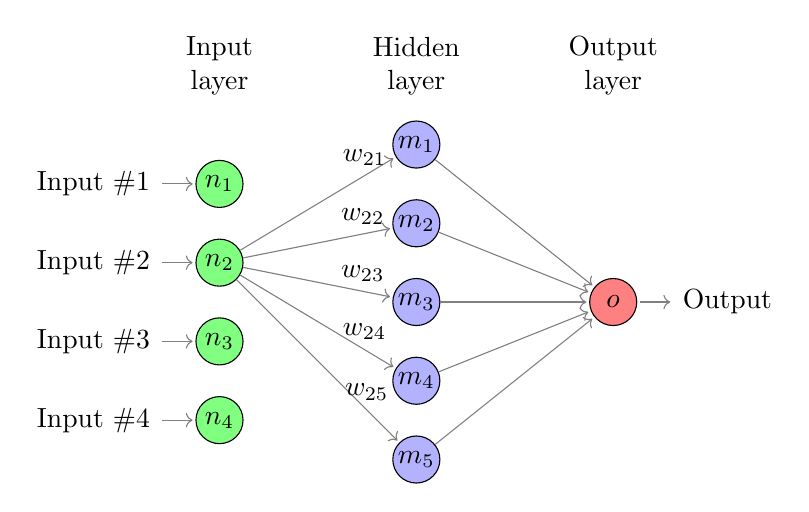
\begin{tikzpicture}[shorten >=1pt,->,draw=black!50, node distance=\layersep]
%https://tex.stackexchange.com/questions/96846/how-to-place-label-in-middle-of-line-above-and-below-with-tikz
    \tikzstyle{every pin edge}=[<-,shorten <=1pt]
    \tikzstyle{neuron}=[circle,fill=black!25,minimum size=17pt,inner sep=0pt, draw=black]
    \tikzstyle{input neuron}=[neuron, fill=green!50];
    \tikzstyle{output neuron}=[neuron, fill=red!50];
    \tikzstyle{hidden neuron}=[neuron, fill=blue!30];
    \tikzstyle{annot} = [text width=4em, text centered]

    % Draw the input layer nodes
    \foreach \name / \y in {1,...,4}
    % This is the same as writing \foreach \name / \y in {1/1,2/2,3/3,4/4}
        \node[input neuron, pin=left:Input \#\y] (I-\name) at (0,-\y) {$n_\y$};

    % Draw the hidden layer nodes
    \foreach \name / \y in {1,...,5}
        \path[yshift=0.5cm]
            node[hidden neuron] (H-\name) at (\layersep,-\y cm) {$m_\y$};

    % Draw the output layer node
    \node[output neuron,pin={[pin edge={->}]right:Output}, right of=H-3] (O) {$o$};

    % Connect every node in the input layer with every node in the
    % hidden layer.
%    \foreach \source in {1,...,4}
%        \foreach \dest in {1,...,5}
%            \draw (I-\source) -- node[below] {$w_ij$} ++ (H-\dest);


%    \foreach \source in {1,...,4}
        \foreach \dest in {1,...,5}
            \draw (I-2) -- node[above, pos=0.8] {$w_{2\dest}$} ++ (H-\dest);

    % Connect every node in the hidden layer with the output layer
    \foreach \source in {1,...,5}
        \path (H-\source) edge (O);

    % Annotate the layers
    \node[annot,above of=H-1, node distance=1cm] (hl) {Hidden layer};
    \node[annot,left of=hl] {Input layer};
    \node[annot,right of=hl] {Output layer};
\end{tikzpicture}
  \end{minipage}
  \vfill
\begin{minipage}[t][0.5\textheight][t]{\textwidth}

\end{minipage}


\end{frame}




\begin{frame}[fragile]{Point Variance of Linear Predictor}

\begin{align*}
\action<+->{ &=&&}
\\
\action<+->{  &=   && }
\end{align*}
\action<+->{The}
\end{frame}



\begin{frame}[fragile]{Correlation}
\begin{itemize}
\item[] \textbf{Serial No.} is basically uncorrelated with anything. \pause
\item[] \textbf{Admit} is highly correlated with \textbf{CGPA}, \textbf{TOEFL Score} and \textbf{GRE Score}\pause
\item[] \textbf{Research} has a lowish correlation with \textbf{Admit}, but also with everything else.  
\end{itemize}
\end{frame}











\begin{frame}[fragile]{Bias, Variance and Parameters}
  \begin{minipage}[t][0.5\textheight][t]{\textwidth}
	\centering
	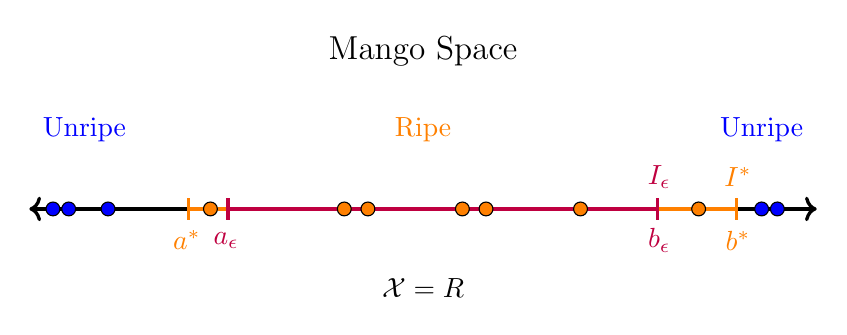
\begin{tikzpicture}
		\draw[<->,very thick] (-5,0) -- (5,0);
		\draw[color = orange, |-|,very thick] (-3,0) -- (4,0);
		\node[color=orange] at (4,.4) {$I^*$};
		\node at (0,2) {\large Mango Space} ;
		\node at (0,-1) {$\mathcal{X} = \mathbb{R}$} ;
		\node [color=blue] at (-4.3,1) {Unripe} ;
		\node [color=blue] at (4.3,1) {Unripe} ;
		\node [color=orange] at (0,1) {Ripe} ;

		\node [color=orange] at (-3,-.4) {$a^*$} ;
		\node [color=orange] at (4,-.4) {$b^*$} ;

		\draw [color=purple, |-|,very thick] (-2.5,0) -- (3,0);
		\node [color=purple] at (3,.4) {$I_\epsilon$} ;
		\node [color=purple] at (-2.5,-.4) {$a_\epsilon$} ;
		\node [color=purple] at (3,-.4) {$b_\epsilon$} ;

%		\draw [color=olive, |-|,very thick] (-3.5,0) -- (2.5,0);
%		\node [color=olive] at (3,.4) {$h_{\mathcal{T}}$} ;



		\node[circle,draw=black, fill=orange, inner sep=0pt,minimum size=5pt] at (2,0) {};
		\node[circle,draw=black, fill=orange, inner sep=0pt,minimum size=5pt] at (-1,0) {};
		\node[circle,draw=black, fill=orange, inner sep=0pt,minimum size=5pt] at (-.7,0) {};
		\node[circle,draw=black, fill=orange, inner sep=0pt,minimum size=5pt] at (.5,0) {};
		\node[circle,draw=black, fill=orange, inner sep=0pt,minimum size=5pt] at (.8,0) {};
		\node[circle,draw=black, fill=orange, inner sep=0pt,minimum size=5pt] at (-2.7,0) {};
		\node[circle,draw=black, fill=orange, inner sep=0pt,minimum size=5pt] at (3.5,0) {};

		\node[circle,draw=black, fill=blue, inner sep=0pt,minimum size=5pt] at (-4.5,0) {};
		\node[circle,draw=black, fill=blue, inner sep=0pt,minimum size=5pt] at (-4,0) {};
		\node[circle,draw=black, fill=blue, inner sep=0pt,minimum size=5pt] at (-4.7,0) {};
		\node[circle,draw=black, fill=blue, inner sep=0pt,minimum size=5pt] at (4.3,0) {};
		\node[circle,draw=black, fill=blue, inner sep=0pt,minimum size=5pt] at (4.5,0) {};
	\end{tikzpicture}
  \end{minipage}
  \vfill
  \begin{minipage}[t][0.5\textheight][t]{\textwidth}
Lets understand this visually.
$$
Err(x_0) = \sigma_\epsilon^2 + [E_\cT[\hat f(x_0)] - f(x_0)]^2 + E_\cT\big[ \hat{f}(x_0) - E_\cT[\hat{f}(x_0)] \big]^2\,.
$$\pause
Consider a data set, 
\end{minipage}
\end{frame}





























